% Archived former Appendix Figure B.2.
\begin{figure}[H]
\centering
\caption{National distributions of household inflation in 2022: RAS, COICOP digit 3}
\label{fig:national-household-inflation-ras-d3}
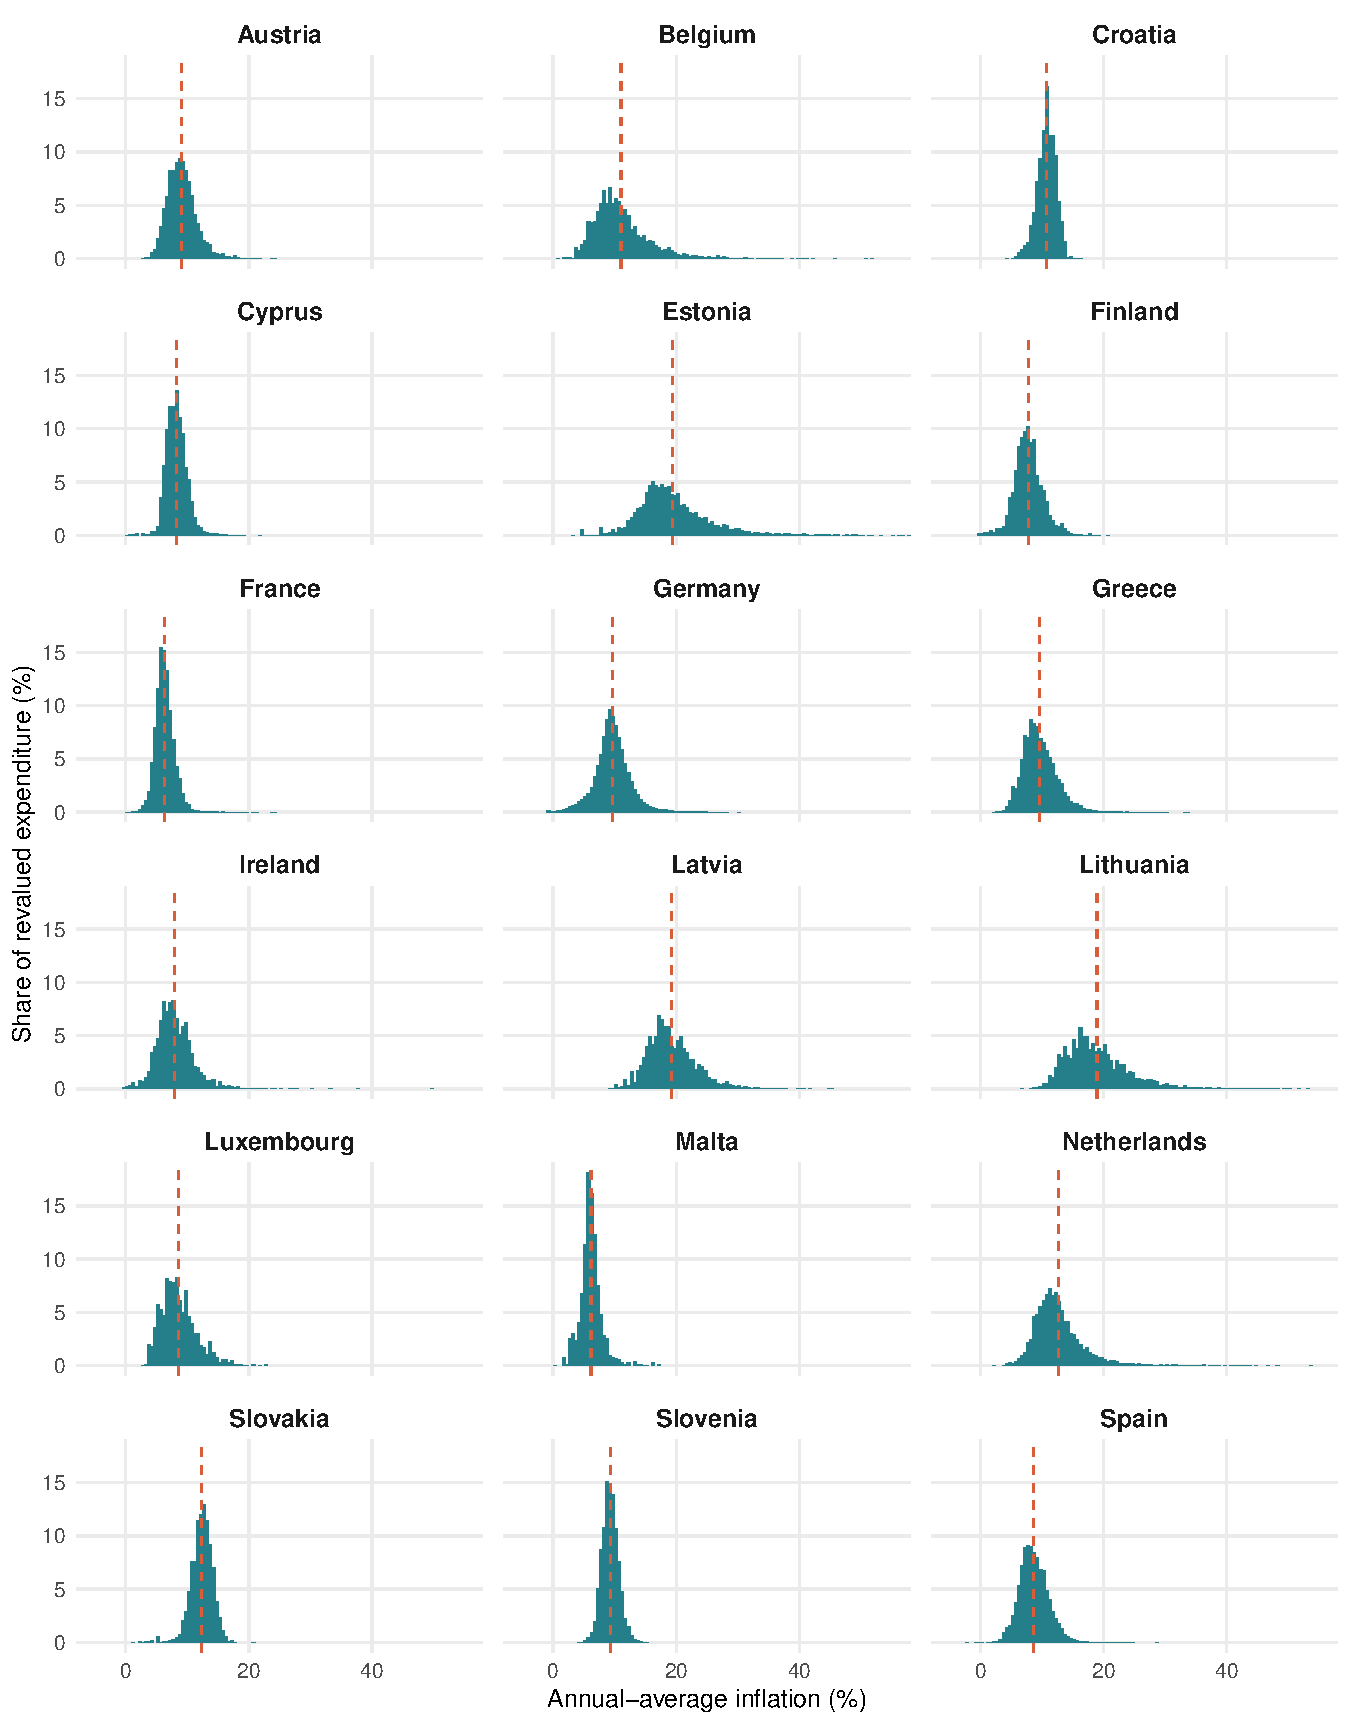
\includegraphics[width=\textwidth,height=0.76\textheight,keepaspectratio]{fig_national_household_inflation_RAS_D3_expenditure_2022.pdf}
\captionsetup{font=footnotesize, format=hang, singlelinecheck=false, justification=justified}
\caption*{Notes: Annual-average inflation; 2020 HBS baskets, excluding rents (041 and 042). Weights equal survey weights times retained expenditure times the 2021 annual-average household index. Orange lines mark the corresponding weighted means. Bins are 0.5 percentage points wide; the displayed range is $-5$ to 55 percent, without renormalization. The expenditure share outside this range is below 0.1 percent in every country. The sample comprises 152,613 households in 18 countries, excluding Italy and Portugal.\\
Sources: HBS microdata, Eurostat HICP; authors' calculations.}
\end{figure}
